\documentclass[compress,red]{beamer}
\usepackage[utf8]{inputenc}
\usepackage{ucs}
\usepackage{amsmath}
\usepackage{amsfonts}
\usepackage{amssymb}
\usepackage[russian]{babel}
\usepackage{graphicx}
\usepackage{wrapfig}

\usepackage{tikz}
\usepackage{verbatim}

\usepackage{color}
\usepackage{xcolor}
\usepackage{listings}

\usepackage{caption}
\DeclareCaptionFont{white}{\color{white}}
\DeclareCaptionFormat{listing}{\colorbox{gray}{\parbox{\textwidth}{#1#2#3}}}
\captionsetup[lstlisting]{format=listing,labelfont=white,textfont=white}

\usetikzlibrary{calc,trees,positioning,arrows,chains,shapes.geometric,%
    decorations.pathreplacing,decorations.pathmorphing,shapes,%
    matrix,shapes.symbols}

\tikzset{
>=stealth',
  punktchain/.style={
    rectangle, 
    rounded corners, 
    % fill=black!10,
    draw=black, very thick,
    text width=10em, 
    minimum height=3em, 
    text centered, 
    on chain},
  line/.style={draw, thick, <-},
  element/.style={
    tape,
    top color=white,
    bottom color=blue!50!black!60!,
    minimum width=8em,
    draw=blue!40!black!90, very thick,
    text width=10em, 
    minimum height=1.5em, 
    text centered, 
    on chain},
  every join/.style={->, thick,shorten <=1pt},
  decoration={brace},
  tuborg/.style={decorate},
  tubnode/.style={midway, right=2pt},
}

\mode<presentation>

\usetheme{Warsaw}

\definecolor{Red}{rgb}{1,0,0}
\definecolor{Blue}{rgb}{0,0,1}
\definecolor{Green}{rgb}{0,1,0}
\definecolor{magenta}{rgb}{1,0,.6}
\definecolor{lightblue}{rgb}{0,.5,1}
\definecolor{lightpurple}{rgb}{.6,.4,1}
\definecolor{gold}{rgb}{.6,.5,0}
\definecolor{orange}{rgb}{1,0.4,0}
\definecolor{hotpink}{rgb}{1,0,0.5}
\definecolor{newcolor2}{rgb}{.5,.3,.5}
\definecolor{newcolor}{rgb}{0,.3,1}
\definecolor{newcolor3}{rgb}{1,0,.35}
\definecolor{darkgreen1}{rgb}{0, .35, 0}
\definecolor{darkgreen}{rgb}{0, .6, 0}
\definecolor{darkred}{rgb}{.75,0,0}

\xdefinecolor{olive}{cmyk}{0.64,0,0.95,0.4}
\xdefinecolor{purpleish}{cmyk}{0.75,0.75,0,0}

\useoutertheme[subsection=false]{smoothbars}


\title{Управляющие структуры в ruby: циклы}
\author{Информатика \\ 10-11 классы}

%\usecolortheme{dolphin}


\begin{document}
%%титульная страница
\maketitle
%% основные моменты

\section{Квадратное уравнение}

\subsection{Описание}
\begin{frame}
  \frametitle{Описание}
  \begin{itemize}
    \item Итак, вернёмся к квадратному уравнению. Напишем программу, высчитывающую все корни (если таковые имеются) квадратного уравнения $ax^2+bx+c=0$.
    \item Если $a \neq 0$, то:
    \begin{enumerate}
      \item Вычислим дискриминант уравнения по формуле: $D = b^2 - 4ac$.
      \item Если дискриминант меньше нуля, то решений нет.
      \item Если дискриминант равен нулю, то корень --- один. Он равен: $-\cfrac{b}{2a}$.
      \item Если дискриминант больше нуля, то существует два вещественных корня:
        \begin{gather*}
          x_{1,2} = \cfrac{-b \pm \sqrt{b^2-4ac}}{2a}
        \end{gather*}
    \end{enumerate}
    \item В случае $a = 0$ уравнение из квадратного превращается в линейное, которое мы уже умеем решать.
  \end{itemize}
\end{frame}

\subsection{Блок--схема}
\begin{frame}
  \frametitle{Блок--схема}
  
  \begin{figure}
  \centering
  \begin{tikzpicture}[node distance=2.0em]
  \tikzset{
      every node/.style={scale=0.6},
      action/.style={rectangle,draw=black, top color=white, bottom color=yellow!50,thin, inner sep=0.25em, minimum size=0.6em, text centered},
      input/.style={ellipse,draw=black, top color=white, bottom color=yellow!50,thin, inner sep=0.25em, minimum size=0.6em, text centered},
      condition/.style={diamond,draw=black, top color=white, bottom color=yellow!50,thin, inner sep=0.25em, minimum size=0.6em, text centered},
      block/.style={chamfered rectangle,draw=black, top color=white, bottom color=yellow!50,thin, inner sep=0.25em, minimum size=0.6em, text centered},
      myarrow/.style={draw},
  }
  \node[input] (item1) {Ввести $a,b,c$};  
  \node[condition, below=0.5em of item1] (item2) {$a == 0$};

  \node (AuxNode01) [text width=0em, left=4.5em of item2] {};
    \node[action, below=of AuxNode01] (item3) {$D = b^2-4ac$};
    \node[condition, below=of item3] (item9) {$D?$};
      \node[action, right=2.5em of item9] (item10) {$x=-\frac{b}{2a}$};
      \node[action, below=1.5em of item9] (item11) {$x_{1,2} = \cfrac{-b\pm \sqrt{D}}{2a}$};
      \node[action, left=2.5em of item9] (item12) {решений нет};

  \node (AuxNode02) [text width=0em, right=3.0em of item2] {};
  \node[condition, below=of AuxNode02] (item4) {$b = 0$};

    \node (AuxNode03) [text width=0cm, left=1.5em of item4] {};
      \node[action, below=of AuxNode03] (item8) {$x = -\frac{c}{b}$};

    \node (AuxNode04) [text width=0cm, right=0.5em of item4] {};
      \node[condition, below=of AuxNode04] (item5) {$c = 0$};
      \node (AuxNode05) [text width=0cm, right=1.0em of item5] {};
        \node[action, below=of AuxNode05] (item6) {любое $x$};
      \node (AuxNode06) [text width=0cm, left=0.5em of item5] {};
        \node[action, below=of AuxNode06] (item7) {решений нет};

  \path[myarrow] (item1) -- (item2);   
  \path[myarrow] (item2) -- node [yshift=1.0em, near start] {нет} (AuxNode01.west);   
  \path[myarrow] (item2) -- node [yshift=1.0em, near start] {да} (AuxNode02.center);   
  \path[myarrow] (AuxNode01.west) -- ++(0,-0.8) (item3);   
  \path[myarrow] (AuxNode02.center) -- (item4);   
    \path[myarrow] (item4.east) -- node [yshift=1.0em, near start] {да} (AuxNode04.center);   
      \path[myarrow] (AuxNode04.center) -- (item5);   
      \path[myarrow] (item5.east) -- node [yshift=1.0em, near start] {да} (AuxNode05.center);   
      \path[myarrow] (AuxNode05.center) -- (item6);   
      \path[myarrow] (item5.west) -- node [yshift=1.0em, near start] {нет} (AuxNode06.center);   
      \path[myarrow] (AuxNode06.center) -- (item7);   
    \path[myarrow] (item4.west) -- node [yshift=1.0em, near start] {нет} (AuxNode03.center);   
    \path[myarrow] (AuxNode03.center) -- (item8);   
  \path[myarrow] (item3.south) -- (item9.north);   
  \path[myarrow] (item9.east) -- node [yshift=1.0em,xshift=0.5em, near start] {$D=0$} (item10.west);   
  \path[myarrow] (item9.south) -- node [yshift=-0.5em,xshift=2.0em, near start] {$D>0$} (item11.north);   
  \path[myarrow] (item9.west) -- node [yshift=1.0em,xshift=-0.5em, near start] {$D<0$} (item12.east);   
  
  \end{tikzpicture} 
  \end{figure}  
  
\end{frame}

\subsection{Программа}
\begin{frame}[fragile]
  \frametitle{Программа}
  \begin{columns}[c]
  \column{2.0in}
    \begin{lstlisting}[language=ruby,basicstyle=\footnotesize,label=ruby1,caption=Квадратное уравнение]
    a = 2.0
    b = 4.0
    c = 2.0
    if (a == 0)
      if (b == 0)
        if (c == 0)
          puts "any x"
        else
          puts "no solutions"
        end
      else
        x = -c/b
        puts x
      end
    else
    \end{lstlisting}
  \column{2.0in}

    \begin{figure}
    \centering
    \begin{tikzpicture}[node distance=2.0em]
    \tikzset{
        every node/.style={scale=0.6},
        action/.style={rectangle,draw=black, top color=white, bottom color=yellow!50,thin, inner sep=0.25em, minimum size=0.6em, text centered},
        input/.style={ellipse,draw=black, top color=white, bottom color=yellow!50,thin, inner sep=0.25em, minimum size=0.6em, text centered},
        condition/.style={diamond,draw=black, top color=white, bottom color=yellow!50,thin, inner sep=0.25em, minimum size=0.6em, text centered},
        block/.style={chamfered rectangle,draw=black, top color=white, bottom color=yellow!50,thin, inner sep=0.25em, minimum size=0.6em, text centered},
        myarrow/.style={draw},
    }
    \node[input] (item1) {Ввести $a,b,c$};  
    \node[condition, below=0.5em of item1] (item2) {$a == 0$};

    \node (AuxNode02) [text width=0em, right=3.0em of item2] {};
    \node[condition, below=of AuxNode02] (item4) {$b = 0$};

      \node (AuxNode03) [text width=0cm, left=1.5em of item4] {};
        \node[action, below=of AuxNode03] (item8) {$x = -\frac{c}{b}$};

      \node (AuxNode04) [text width=0cm, right=0.5em of item4] {};
        \node[condition, below=of AuxNode04] (item5) {$c = 0$};
        \node (AuxNode05) [text width=0cm, right=1.0em of item5] {};
          \node[action, below=of AuxNode05] (item6) {любое $x$};
        \node (AuxNode06) [text width=0cm, left=0.5em of item5] {};
          \node[action, below=of AuxNode06] (item7) {решений нет};

    \path[myarrow] (item1) -- (item2);   
    \path[myarrow] (item2) -- node [yshift=1.0em, near start] {да} (AuxNode02.center);   
    \path[myarrow] (AuxNode02.center) -- (item4);   
      \path[myarrow] (item4.east) -- node [yshift=1.0em, near start] {да} (AuxNode04.center);   
        \path[myarrow] (AuxNode04.center) -- (item5);   
        \path[myarrow] (item5.east) -- node [yshift=1.0em, near start] {да} (AuxNode05.center);   
        \path[myarrow] (AuxNode05.center) -- (item6);   
        \path[myarrow] (item5.west) -- node [yshift=1.0em, near start] {нет} (AuxNode06.center);   
        \path[myarrow] (AuxNode06.center) -- (item7);   
      \path[myarrow] (item4.west) -- node [yshift=1.0em, near start] {нет} (AuxNode03.center);   
      \path[myarrow] (AuxNode03.center) -- (item8);   
  
    \end{tikzpicture} 
    \end{figure}

  \end{columns}
  
\end{frame}

\subsection{Программа}
\begin{frame}[fragile]
  \frametitle{Программа}
  \begin{columns}[c]
  \column{2.0in}
    \begin{lstlisting}[language=ruby,basicstyle=\footnotesize,label=ruby2,caption=Квадратное уравнение]

    else
      D = b*b-4*a*c
      if (D > 0)
        x1 = (-b+D**0.5)/(2.0*a)
        x2 = (-b-D**0.5)/(2.0*a)
        puts x1,x2
      elsif (D == 0)
        x = -b/(2*a)
        puts x
      else
        puts "no solutions"
      end
    end
    \end{lstlisting}
  \column{2.0in}
  
    \begin{figure}
    \centering
    \begin{tikzpicture}[node distance=2.0em]
    \tikzset{
        every node/.style={scale=0.6},
        action/.style={rectangle,draw=black, top color=white, bottom color=yellow!50,thin, inner sep=0.25em, minimum size=0.6em, text centered},
        input/.style={ellipse,draw=black, top color=white, bottom color=yellow!50,thin, inner sep=0.25em, minimum size=0.6em, text centered},
        condition/.style={diamond,draw=black, top color=white, bottom color=yellow!50,thin, inner sep=0.25em, minimum size=0.6em, text centered},
        block/.style={chamfered rectangle,draw=black, top color=white, bottom color=yellow!50,thin, inner sep=0.25em, minimum size=0.6em, text centered},
        myarrow/.style={draw},
    }
    \node[condition] (item2) {$a == 0$};

    \node (AuxNode01) [text width=0em, left=4.5em of item2] {};
      \node[action, below=of AuxNode01] (item3) {$D = b^2-4ac$};
      \node[condition, below=of item3] (item9) {$D?$};
        \node[action, right=2.5em of item9] (item10) {$x=-\frac{b}{2a}$};
        \node[action, below=1.5em of item9] (item11) {$x_{1,2} = \cfrac{-b\pm \sqrt{D}}{2a}$};
        \node[action, left=2.5em of item9] (item12) {решений нет};

    \path[myarrow] (item2) -- node [yshift=1.0em, near start] {нет} (AuxNode01.west);   
    \path[myarrow] (AuxNode01.west) -- ++(0,-0.8) (item3);   
    \path[myarrow] (item3.south) -- (item9.north);   
    \path[myarrow] (item9.east) -- node [yshift=1.0em,xshift=0.5em, near start] {$D=0$} (item10.west);   
    \path[myarrow] (item9.south) -- node [yshift=-0.5em,xshift=2.0em, near start] {$D>0$} (item11.north);   
    \path[myarrow] (item9.west) -- node [yshift=1.0em,xshift=-0.5em, near start] {$D<0$} (item12.east);   
  
    \end{tikzpicture} 
    \end{figure}  
  
  \end{columns}
\end{frame}

\section{Циклы}
\subsection{Основы}
\begin{frame}[fragile]
  \frametitle{Основы}
		\begin{itemize}
  		\item Часто встречаются ситуации, когда какое-либо действие надо повторить несколько раз.
  		\item Например, вывести на экран первые 5 натуральных чисел.
  		\item Простейшая программа выглядела бы следующим образом:
  	\end{itemize}
  	
    \begin{lstlisting}[language=ruby,label=ruby3,caption=5 последовательных чисел]
      puts "1,2,3,4,5"
    \end{lstlisting}		
    
		\begin{itemize}
  	  \item А если чисел — 100? 1000? 10000?
		\end{itemize}
\end{frame}

\subsection{Основы}
\begin{frame}[fragile]
  \frametitle{Основы}
		\begin{itemize}
  		\item На помощь приходят \emph{циклы}.
  		\item \emph{Цикл} --- управляющая структура в алгоритме/программе, позволяющая повторять какую-либо операцию несколько раз.
  		\item Два основных типа циклов:
  		  \begin{enumerate}
  		    \item с заданным количеством шагов--итераций (\emph{явный цикл})
  		    \item без явно заданного количества итераций (\emph{неявный цикл})
  		  \end{enumerate}
  		\item Первый тип состоит из начала цикла, номера итерации, тела цикла (что делаем), конца цикла.
  		\item Второй тип — из начала цикла, условия выхода из цикла, номера итерации (опционально), тела цикла, конца цикла.
  	\end{itemize}
\end{frame}

\subsection{Неявный цикл}
\begin{frame}
  \frametitle{Пример цикла}
	\centerline{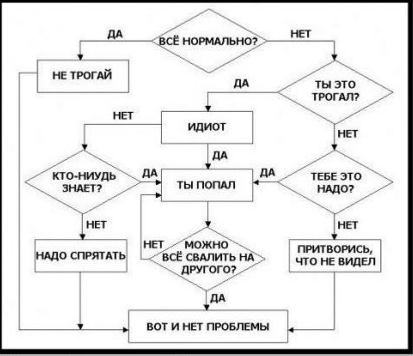
\includegraphics[width=0.7\textwidth]{images/how_to_fix_a_problem.png}\footnote{Где здесь цикл и какому типу он принадлежит?}}
\end{frame}

\subsection{For и while}
\begin{frame}[fragile]
  \frametitle{For и while}
		\begin{itemize}
  		\item Двум типам циклов соответствует два оператора: \emph{for} и \emph{while}.
  		\item Напишем программу, выводящую на экран числа от 1 до 100.
  	\end{itemize}
  	
    \begin{columns}[t]
    \column{2.0in}
      \begin{lstlisting}[language=ruby,numbersep=2pt,basicstyle=\footnotesize,label=ruby4,caption=for]
        for i in 1..100
          puts i
        end
      \end{lstlisting}
    \column{2.0in}
      \begin{lstlisting}[language=ruby,basicstyle=\footnotesize,label=ruby5,caption=while]
        i = 0
        while (i < 100)
          i = i+1
          puts i
        end
      \end{lstlisting}
    \end{columns}  	
\end{frame}

\subsection{For и while}
\begin{frame}[fragile]
  \frametitle{For и while}
		\begin{itemize}
  		\item Рассмотрим программы более детально.
  		\item Оба оператора образуют следующую структуру:
  		  \begin{enumerate}
  		    \item Ключевое слово (\textbf{for} или \textbf{while}).
  		    \item Условие повторения (явное или неявное).
  		    \item Конец (оператор \textbf{end}).
  		  \end{enumerate}
  		\item В определении цикла for используется специальная переменная \emph{i}, которая указывает на номер итерации.
  		\item Она ``пробегает'' значения в заданном интервале: for~i~in~1..100 последовательно пробегает значения 1, 2, 3, ... 99, 100.
  		\item В цикле while с помощью оператора присваивания (i~=~i+1) мы \emph{эмулируем} такую переменную.
  	\end{itemize}
\end{frame}

\section{Задачи на циклы}

\subsection{Сумма чисел от 1 до 10000}
\begin{frame}[fragile]
  \frametitle{Суммирование чисел: алгоритм}
		\begin{itemize}
  		\item Посчитаем сумму чисел от 1 до 100000 с помощью циклов.
  	\end{itemize}
  	
  	\begin{columns}[t]
    \column{2.0in}
      \center{\textbf{For}}
      \begin{figure}
      \centering
      \begin{tikzpicture}[node distance=2.0em]
      \tikzset{
          every node/.style={scale=0.6},
          action/.style={rectangle,draw=black, top color=white, bottom color=yellow!50,thin, inner sep=0.25em, minimum size=0.6em, text centered},
          input/.style={ellipse,draw=black, top color=white, bottom color=yellow!50,thin, inner sep=0.25em, minimum size=0.6em, text centered},
          condition/.style={diamond,draw=black, top color=white, bottom color=yellow!50,thin, inner sep=0.25em, minimum size=0.6em, text centered},
          block/.style={chamfered rectangle,draw=black, top color=white, bottom color=yellow!50,thin, inner sep=0.25em, minimum size=0.6em, text centered},
          myarrow/.style={draw},
      }
      
      \node (AuxNode01) [text width=0em] {};
      \node[block, below=1.0em of AuxNode01] (item1) {по i от 1 до 100000};
      \node[action, below right=1.0em of item1] (item2) {sum:=sum+i};
      \node (AuxNode02) [text width=0em, below=1.0em of item2] {};
      \node (AuxNode03) [text width=0em, left=4.0em of AuxNode02] {};
      \node (AuxNode04) [text width=0em, left=4.0em of AuxNode03] {};
      \node (AuxNode05) [text width=0em, left=0.6em of item1] {};
      \node (AuxNode06) [text width=0em, below=1.0em of AuxNode03] {};

      \path[myarrow] (AuxNode01.center) -- (item1.north);   
      \path[myarrow] (item1.east) -| (item2.north);   
      \path[myarrow] (item2.south) -- (AuxNode02.center);   
      \path[myarrow] (AuxNode02.center) -- (AuxNode03.center);   
      \path[myarrow] (AuxNode03.center) -- (AuxNode04.center);   
      \path[myarrow] (AuxNode04.center) -- (AuxNode05.center);   
      \path[myarrow] (AuxNode05.center) -- (item1.west);   
      \path[myarrow] (AuxNode03.center) -- (AuxNode06.center);   
  
      \end{tikzpicture} 
      \end{figure}

    \column{2.0in}
      \center{\textbf{While}}
      \begin{figure}
      \centering
      \begin{tikzpicture}[node distance=2.0em]
      \tikzset{
          every node/.style={scale=0.6},
          action/.style={rectangle,draw=black, top color=white, bottom color=yellow!50,thin, inner sep=0.25em, minimum size=0.6em, text centered},
          input/.style={ellipse,draw=black, top color=white, bottom color=yellow!50,thin, inner sep=0.25em, minimum size=0.6em, text centered},
          condition/.style={diamond,draw=black, top color=white, bottom color=yellow!50,thin, inner sep=0.25em, minimum size=0.6em, text centered},
          block/.style={chamfered rectangle,draw=black, top color=white, bottom color=yellow!50,thin, inner sep=0.25em, minimum size=0.6em, text centered},
          myarrow/.style={draw},
      }
    
      \node (AuxNode01) [text width=0em] {};
      \node[condition, below=1.0em of AuxNode01] (item1) {i<=100000};
      \node[action, below=1.0em of item1] (item2) {i:=i+1};
      \node[action, below=1.0em of item2] (item3) {sum:=sum+i};
      \node (AuxNode03) [text width=0em, left=2.0em of item3] {};
      \node (AuxNode02) [text width=0em, right=1.0em of item1] {};

      \path[myarrow] (AuxNode01.center) -- (item1.north);   
      \path[myarrow] (item1.south) -- node [xshift=1.0em, yshift=-0.5em, near start] {да} (item2.north);   
      \path[myarrow] (item1.east) -- node [yshift=0.5em, xshift=0.5em, near start] {нет} (AuxNode02.center);   
      \path[myarrow] (item2.south) -- (item3.north);   
      \path[myarrow] (item3.west) -- (AuxNode03.center);   
      \path[myarrow] (AuxNode03.center) |- (item1.west);   

      \end{tikzpicture} 
      \end{figure}

    \end{columns}
\end{frame}

\subsection{Сумма чисел от 1 до 100000}
\begin{frame}[fragile]
  \frametitle{Программа}
  	\begin{columns}[t]
    \column{2.0in}
      \begin{lstlisting}[language=ruby,numbersep=2pt,basicstyle=\footnotesize,label=ruby6,caption=for]
        sum = 0
        for i in 1..100000
          sum = sum + i
        end
        puts sum
      \end{lstlisting}
    \column{2.0in}
      \begin{lstlisting}[language=ruby,basicstyle=\footnotesize,label=ruby7,caption=while]
        i   = 0
        sum = 0
        while (i < 100000)
          i = i+1
          sum = sum + i
        end
        puts sum
      \end{lstlisting}
    \end{columns}
\end{frame}

\subsection{Логарифм}
\begin{frame}[fragile]
  \frametitle{Логарифмирование}
		\begin{itemize}
  		\item Задача: найти наименьшее целое число, для которого выполнено неравенство:
  		  \begin{gather*}
  		    2^x > 1000000
		    \end{gather*}
		  \item Цикл \emph{for} здесь не поможет, ведь мы заранее не знаем, сколько итераций будет.
		  \item Решаем через \emph{while}. Как?
		  \item Пробежим все степени двойки, начиная с нулевой, фиксируя на каждом шаге значение показателя степени.
		  \item Если текущее значение меньше 1000000, увеличим показатель на 1.
		  \item Когда-нибудь наступит ситуация, когда 2 в какой-либо степени станет больше, чем 1000000. 
		  \item Последнее значение показателя степени и будет искомым числом.
  	\end{itemize}
\end{frame}

\subsection{Логарифм}
\begin{frame}[fragile]
  \frametitle{Логарифмирование}

    \begin{lstlisting}[language=ruby,numbersep=2pt,label=ruby9,caption=Вычисление наименьшей степени]
      num = 0
      i = 0
      while (num <= 1000000)
        i = i+1
        num = 2**i
      end
      puts i
    \end{lstlisting}
    \begin{itemize}
      \item Задание: дан алфавит, состоящий из N букв. Написать программу, которая считает, сколько бит занимает один символ этого алфавита.
    \end{itemize}
\end{frame}

\subsection{Выход из цикла}
\begin{frame}[fragile]
  \frametitle{Выход из цикла}
  \begin{itemize}
    \item Может возникнуть ситуация, когда нам нужно прекратить выполнение до цикла даже несмотря на то, что не все итерации пройдены.
    \item Для окончания цикла нужно вызвать оператор \textbf{break}.
    \item Пример: если бы в задаче $2^x > 1000000$ мы использовали цикл for, то нам следовало бы остановиться в ситуации, когда $2^i$ стало бы больше 1000000, где $i$ --- номер итерации.
  \end{itemize} 
  \begin{lstlisting}[language=ruby,basicstyle=\footnotesize,numbersep=2pt,label=ruby11,caption=Break]
    for i in 1..1000000
      ...
      break if (2**i > 1000000)
    end
  \end{lstlisting}
  \begin{itemize}
    \item Для перехода к следующей итерации без выполнения дальнейшего кода из тела цикла --- оператор \textbf{next}.
  \end{itemize}
\end{frame}

\subsection{Times}
\begin{frame}[fragile]
  \frametitle{Оператор times}
  \begin{itemize}
    \item Оператор \textbf{times} (\emph{англ.} кол-во раз) очень похож на \textbf{for}. Он повторяет определённое заданное количество раз определённое действие.
    \item Его зачастую используют, когда цикл --- очень простой и содержит всего одно действие.
    \item Приведём пример: выведем на экран квадраты чисел от 0 до 9.
  \end{itemize}
  \begin{lstlisting}[language=ruby,numbersep=2pt,label=ruby10,caption=Вычисление наименьшей степени]
    10.times { |i| puts i**2 }
  \end{lstlisting}
  \begin{itemize}
    \item Лаконично, не правда ли?
    \item NB! Нумерация начинается с 0, а не с 1!
  \end{itemize}
  
\end{frame}

\section{Числа Фибоначчи}
\subsection{Числа Фибоначчи}
\begin{frame}[fragile]
  \frametitle{Числа Фибоначчи}
	\begin{itemize}
		\item \emph{Числа Фибоначчи} задаются \emph{рекуррентной} формулой:
		  \begin{gather*}
		    \varphi_n = \varphi_{\rm{n}-1}+\varphi_{\rm{n}-2}
		  \end{gather*}
		  где $\varphi_0 = 1, \varphi_1 = 1$.
		\item Первые несколько чисел Фибоначчи:
		  \begin{tabular}{|c|c|c|c|c|c|c|c|c|c|c|}
		  \hline
		  $\varphi_0$ & $\varphi_1$ & $\varphi_2$ & $\varphi_3$ & $\varphi_4$ & $\varphi_5$ & $\varphi_6$ & $\varphi_7$ & $\varphi_8$ & $\varphi_9$ & $\varphi_{10}$ &  
		  \hline
		  1 & 1 & 2 & 3 & 5 & 8 & 13 & 21 & 34 & 55 & 89 \\
		  \hline
		  \end{tabular}
		\item Числа Фибоначчи встречаются и в природе: филлотаксис (листорасположение) у растений описывается последовательностью Фибоначчи. 
		\item Зерна подсолнуха, сосновые шишки, лепестки цветков располагаются также по числам Фибоначчи.
  \end{itemize}  
\end{frame}

\subsection{Числа Фибоначчи}
\begin{frame}
  \frametitle{Числа Фибоначчи}
	\centerline{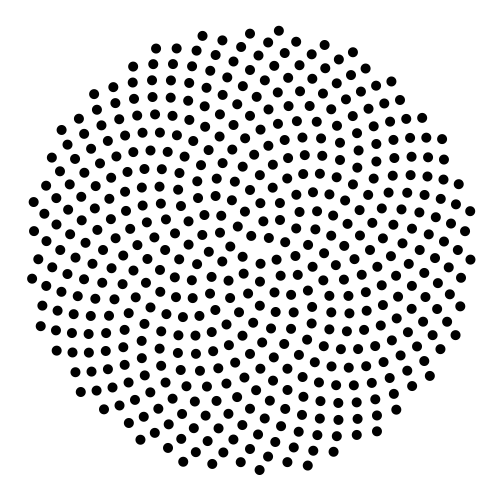
\includegraphics[width=0.7\textwidth]{images/sunflower1.png}}
\end{frame}

\subsection{Числа Фибоначчи}
\begin{frame}
  \frametitle{Числа Фибоначчи}
	\centerline{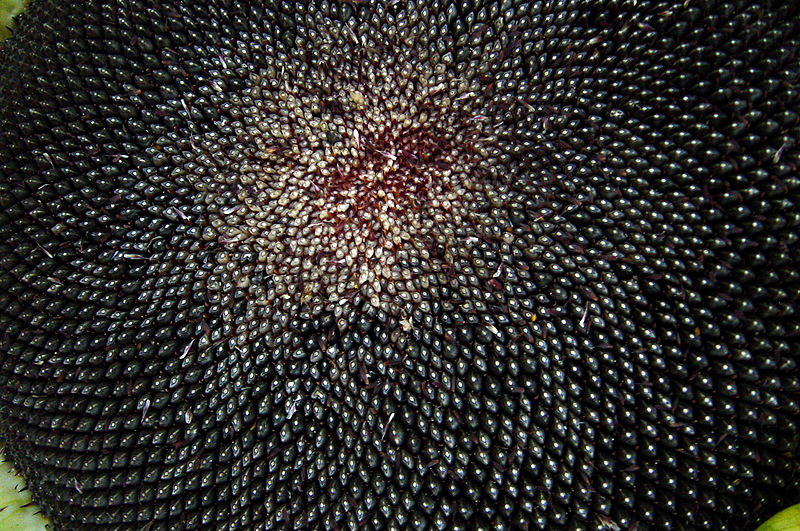
\includegraphics[width=0.7\textwidth]{images/sunflower2.png}}
\end{frame}

\subsection{Числа Фибоначчи}
\begin{frame}[fragile]
  \frametitle{Вычисление 100 числа Фибоначчи }
	\begin{itemize}
	  \item Итак, чтобы вычислить число Фибоначчи, нужно знать два предыдущих.
	  \item Пойдём последовательно. Нам известны значения двух первых чисел: $\varphi_0 = 1, \varphi_1 = 1$.
	  \item Чтобы вычислить второе число, надо сложить первое и нулевое.
	  \item Прибавив к полученному числу первое — получим третье:
	    \begin{gather*}
	      \varphi_3 = \varphi_2 + \varphi_1 = (\varphi_1 + \varphi_0) + \varphi_0.
	    \end{gather*}
	  \item Для вычисления четвёртого числа воспользуемся значениями третьего и второго.
	  \item Итого: нам надо хранить два последних числа. Складывая их, мы получаем новое число. ``Сдвигаемся'' на единицу дальше.
  \end{itemize}
\end{frame}

\subsection{Числа Фибоначчи}
\begin{frame}[fragile]
  \frametitle{Программа}
    \begin{lstlisting}[language=ruby,numbersep=2pt,label=ruby12,caption=100 число Фибоначчи]
      a0 = 1
      a1 = 1
      a_new = 0
      for i in 2..100
        a_new = a0 + a1
        a0 = a1
        a1 = a_new
      end
      puts a_new
    \end{lstlisting}
    \begin{itemize}
      \item Задание: подготовить блок--схему программы.
      \item Задание: сделать аналогично с циклом \emph{while}.
    \end{itemize}
\end{frame}

\subsection{References}
\begin{frame}[fragile]
  \frametitle{References}
  \begin{itemize}
    \item Все презентации доступны на http://school.smirik.ru!
    \item Вопросы, предложения, д/з: smirik@gmail.com
  \end{itemize}
\end{frame}


\end{document}